\documentclass[12pt]{article}
\usepackage[top=1in,left=1in, right = 1in, footskip=1in]{geometry}

\usepackage{graphicx}
%\usepackage{adjustbox}

\newcommand{\eref}[1]{(\ref{eq:#1})}
\newcommand{\fref}[1]{Fig.~\ref{fig:#1}}
\newcommand{\Fref}[1]{Fig.~\ref{fig:#1}}
\newcommand{\sref}[1]{Sec.~\ref{#1}}
\newcommand{\frange}[2]{Fig.~\ref{fig:#1}--\ref{fig:#2}}
\newcommand{\tref}[1]{Table~\ref{tab:#1}}
\newcommand{\tlab}[1]{\label{tab:#1}}
\newcommand{\seminar}{SE\mbox{$^m$}I\mbox{$^n$}R}

\usepackage{amsthm}
\usepackage{amsmath}
\usepackage{amssymb}
\usepackage{amsfonts}

\usepackage{lineno}
%\linenumbers

\usepackage[pdfencoding=auto, psdextra]{hyperref}

\bibliographystyle{chicago}
\usepackage{natbib}
\date{\today}

\usepackage{xspace}
\newcommand*{\ie}{i.e.\@\xspace}

\usepackage{color}

\newcommand{\Rx}[1]{\ensuremath{{\mathcal R}_{#1}}} 
\newcommand{\Ro}{\Rx{0}}
\newcommand{\RR}{\ensuremath{{\mathcal R}}}
\newcommand{\Rhat}{\ensuremath{{\hat\RR}}}
\newcommand{\tsub}[2]{#1_{{\textrm{\tiny #2}}}}

\newcommand{\comment}[3]{\textcolor{#1}{\textbf{[#2: }\textsl{#3}\textbf{]}}}
\newcommand{\jd}[1]{\comment{cyan}{JD}{#1}}
\newcommand{\swp}[1]{\comment{magenta}{SWP}{#1}}
\newcommand{\dc}[1]{\comment{blue}{DC}{#1}}
\newcommand{\hotcomment}[1]{\comment{red}{HOT}{#1}}

\newcommand{\jdnew}{\jd{NEW}}
\newcommand{\jddel}[1]{\jd{DELETE: #1}}

\begin{document}

\begin{flushleft}{
	\Large
	\textbf\newline{
		Modeling the spread of SARS-CoV-2 on a university campus: lessons from Princeton University
	}
}
\newline
\\ 

\end{flushleft} 

\pagebreak

\section{Introduction}

Predicting and controlling the spread of SARS-CoV-2 remains a critical question as new variants continue to emerge and become dominant.
Throughout the pandemic, testing of both asymptomatic and symptomatic individuals has 

University campuses provide unique test cases for understanding the 


- Usual pandemic start

- modeling, understanding control
- testing frequency is important
- universities provide a particularly test case; asymptomatic infection and testing is very high

- little review of what other universities have done

- epideimc in relatively well controlled documented setting
- really well until omicron
- perhaps because of immunity waning 

\section{Methods}

\subsection{Data descriptions}

\begin{figure}[!th]
\includegraphics[width=\textwidth]{../figure_princeton/figure_princeton.pdf}
\caption{
\textbf{Dynamics of SARS-CoV-2 outbreaks in Princeton University}
(A--C) Epidemic trajectories across three semesters: Fall 2020 (A), Spring 2020 (B), and Fall 20201 (C).
Colored bar plots represent the weekly number of cases from both asymptomatic and symptomatic testing in Princeton University.
Red lines represent the weekly number of cases in Mercer County.
Number of cases in Mercery County is obtained from \url{https://github.com/nytimes/covid-19-data}.
(D--F) Correlations between the weekly number of cases in Princeton University and in Mercer County.
Solid lines and shaded areas represent the estimated lienar regression lines and the associated 95\% CIs.
\label{fig:princeton}
}
\end{figure}

We analyze time series of COVID-19 case reports from Princeton University (\fref{princeton}A--C).
Princeton University is located in Mercer County, New Jersey, USA and consists of roughly 5000 undergraduate students, 3000 graduate students, and 7000 staffs and faculties.
All data are publicly available on Princeton University COVID-19 Dashboard website: \url{https://covid.princeton.edu/dashboard}.
We also analyze time series of COVID-19 case reports from Mercer County, New Jersey, USA to compare the levels of community (\fref{princeton}D--F);
these data are taken from the COVID-19 data repository provided by New York Times (\url{https://github.com/nytimes/covid-19-data}).
We aggregate data at a weekly level to remove changes in testing patterns throughout a week.

For simplicity, we divide the time series into three time periods representing three semesters: Fall 2020 (August 24, 2020--January 1, 2021; \fref{princeton}A), Spring 2020 (January 16, 2021--May 14, 2021; \fref{princeton}B), and Fall 2021 (August 14, 2021--December 24, 2021; \fref{princeton}C).
Throughout the study period, all students, staff and faculty members who were physically present for more than 8 hours on campus per week were required to asymptomatic testing with varying frequencies.
Asymptomatic individuals submitted self-collected saliva samples, from which the presence of SARS-CoV-2 was tested using Polymerase Chain Reaction (PCR) \swp{regular PCR? RT-PCR? what are we using?}.  
Asymptomatic individuals who tested positive were required to isolate for 10 days.
Symptomatic individuals were eligible for rapid PCR tests and had to isolate \swp{self-isolate?} until they received their test results---those who tested positive were required to isolate for at least 10 days after symptom onset ond were release 3 days after symptoms resolved.

During fall 2020, roughly 1000 grad students and 2000 staffs and faculties were present on campus and were subject to asymptomatic testing. 
Undergraduate students were not allowed to return back to campus, and so their numbers were minimal (<300).  
Both undergraduate students and graduate students were required to get tested twice a week, whereas staffs and faculties were required to get tested once a week.
The number of cases remained relatively low throughout the semester with peak occuring in early December (\fref{princeton}A), coinciding with the epidemic trajectory in Mercer County (\fref{princeton}D).
We note that a sudden decrease in the number of cases around Thanksgiving may reflect reduced number of tests (3852 and 2972 asymptomatic tests performed on the week ending November 20th and 27th, respectively) as well as actual transmission.
The highest number of cases was reported among staffs and faculties (169), followed by graduate students (41), and undergraduate students (4).

In the beginning of spring 2020, the number of cases suddenly increased before classes began (\fref{princeton}B), reflecting $\approx 3000$ undergraduate students returning to campus.
The classes remained virtual and testing protocol did not change (twice a week for undergraduate and graduate students, and once a week for staffs and faculties).
The number of cases persisted at similar levels as the fall semester and eventually decreased as classes ended and students went back home.
The highest number of cases was reported among staffs and faculties (111), followed by undergraduate students (101), and graduate students (29).

In fall 2021, all students, staffs, and faculties were required to be vaccinated \swp{with two doses?} with a very few exceptions for medical and religious reasons. 
By the beginning of the semesters, ??\% of students and ??\% of staffs and faculties were vaccinated.
As of January 11th, 99\% of undergraduate students, 98\% of graduate students, and 96\% of staffs and faculties have been vaccinated.
Vaccinated individuals were required to be tested once a week, while unvaccinated individuals were required to be tested twice a week.
In-person teaching and activities were allowed on campus.
Everyone was required to wear masks indoors with a few exceptions (e.g., when eating or drinking, or when teaching a small class).
The number of cases remained similar to previous semesters until November when the number of cases began to increase primarily among undergraduate students around Thanksgiving (\fref{princeton}C).  
On November 27th, 2021, Princeton University announced undergraduate students to be tested twice a week and limited the size of non-academic gatherings to 20 people.
The number of cases decreased slightly as classes ended but soon increased back up as the Omicron variant was introduced.

\subsection{Mathematical model}

Throughout the pandemic, mathematical models were used to inform policy decisions, including the frequency of asymptomatic tests.



\section{Results}

\section{Discussion}


\pagebreak

\begin{figure}[!th]
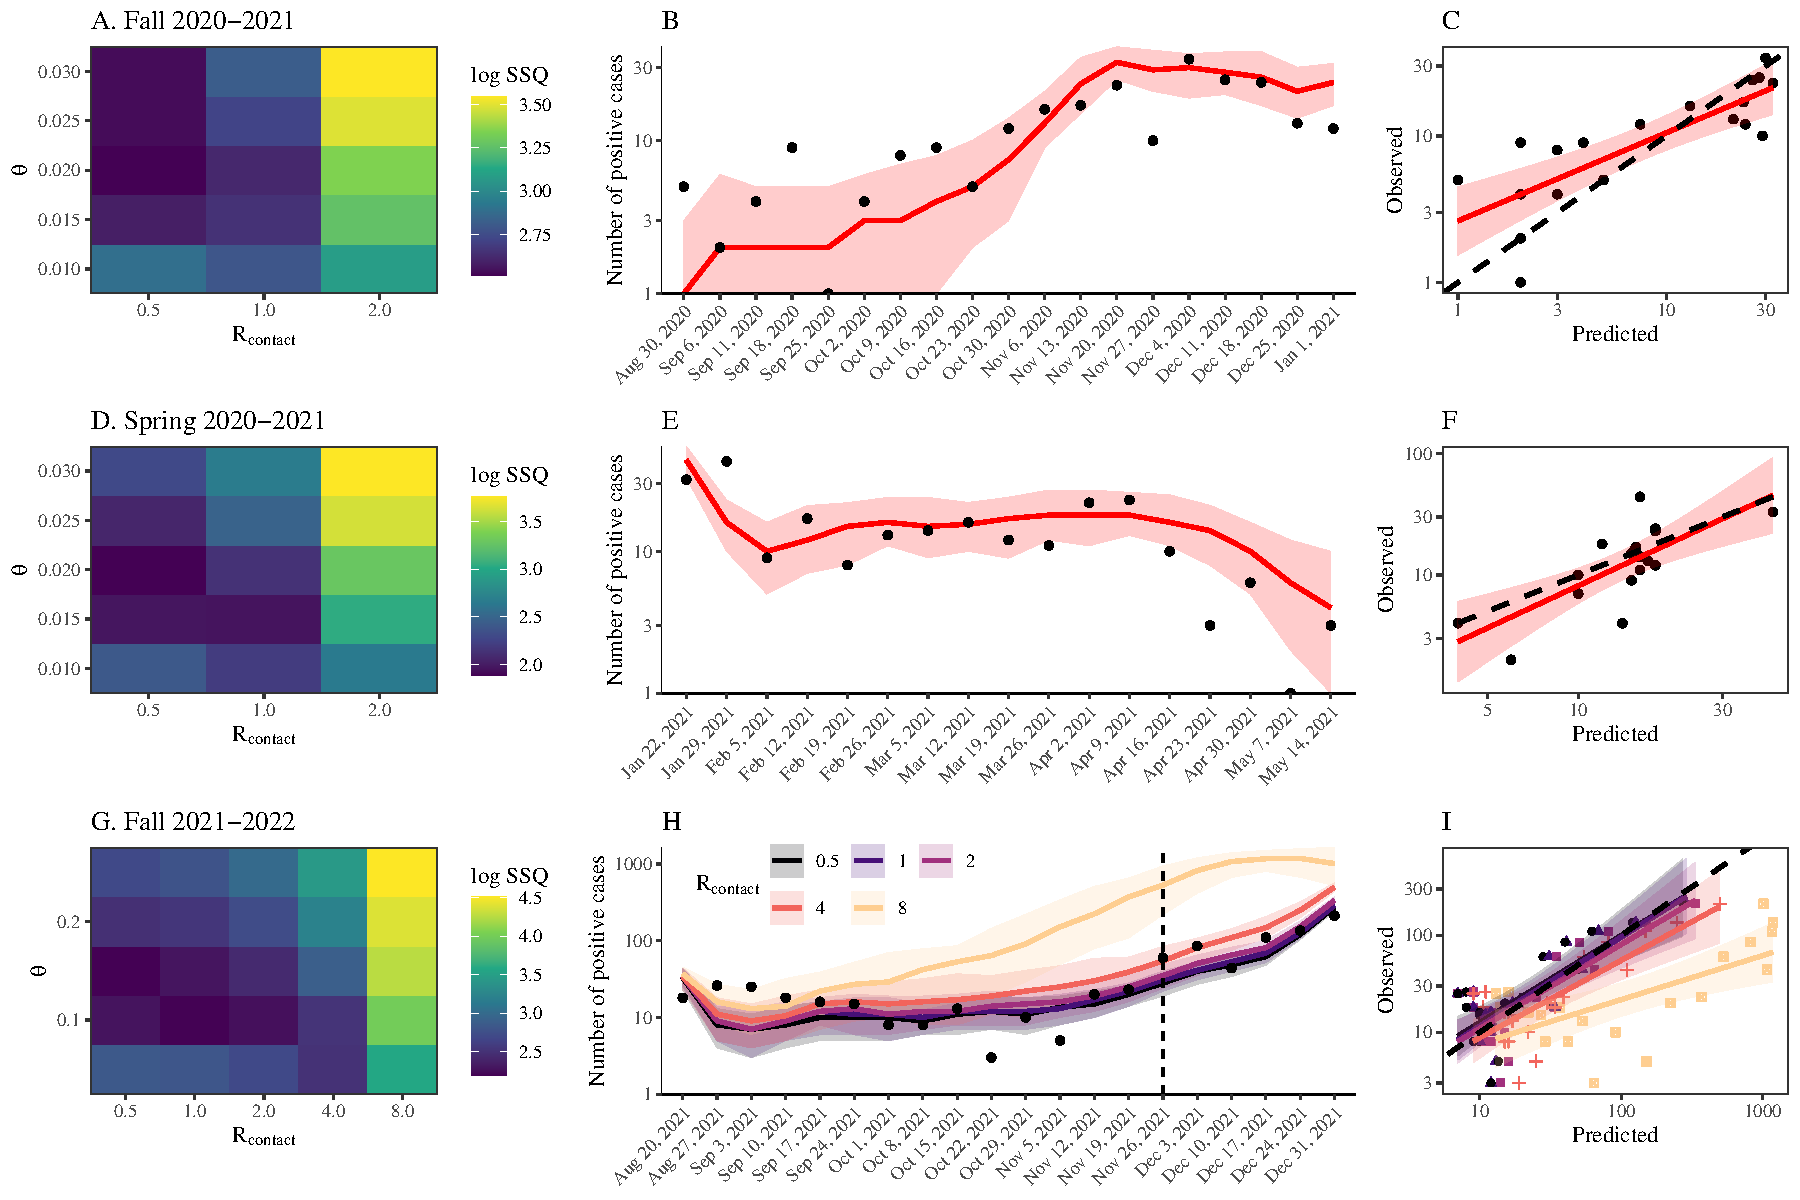
\includegraphics[width=\textwidth]{../figure_princeton/figure_princeton_simulation.pdf}
\caption{
\textbf{Dynamics of SARS-CoV-2 outbreaks in Princeton University}
(A, D, G) Time series comparisons of model predictions with observed data across ranges of paramters: basic reproduction number $\mathcal R_0$, scaling parameter for community transmission $\theta$, and the initial proportion of infected individuals $I_0$.
For each paramter combination, we simulate the model 100 times and calculate the sum of squared differences (SSQ) between the reported number of positive cases and the model-predicted number of positive cases. 
Heatmaps represent medians of the logged sum of squared differences.
(B, E, H) Model predictions. 
Solid lines represent median predictions.
Shaded areas represent 90\% quantiles for the best matching parameter set.
Points represent the observed data.
(C, F, I) Correlations between model predictions with observed data.
Colored solid lines and shaded areas represent the estimated lienar regression lines and the associated 95\% CIs.
Dashed lines represent the one-to-one line.
}
\end{figure}

\pagebreak

\begin{figure}[!th]
\includegraphics[width=\textwidth]{../figure_omicron/figure_omicron.pdf}
\caption{
\textbf{Scenario projects of the spread of omicron variant on university campus}
(A) The predicted daily number of new infections across a wide ranges assumptions about testing frequencies, basic reproduction number $\mathcal R_0$, and the number of booster shots given per day.
(B) The predicted effective susceptibility over time. 
Effective susceptibility is calculated by taking the mean of individual-level susceptibility of each student.
Solid lines and shaded areas represent the median and the corresponding 90\% quantiles across 100 simulations.
All other parameters are the same as in Figure 2.
}
\end{figure}


\pagebreak

\begin{figure}[!th]
\includegraphics[width=\textwidth]{../figure_omicron/figure_omicron_limit.pdf}
\caption{
\textbf{Scenario projects of the spread of omicron variant on university campus with limited isolation beds}
(A) The predicted numbers of individuals in isolation on a given day.
(B) The predicted daily number of new infections.
Solid lines and shaded areas represent the median and the corresponding 90\% quantiles across 100 simulations.
We assume $\mathcal R_0 = 8$, 30 booster shots given per day, and testing frequency of 3 days for these simulations.
All other parameters are the same as in Figure 3.
}
\end{figure}


\end{document}
